\usepackage{amsmath,amssymb,graphicx,alltt}
\DeclareGraphicsRule{*}{mps}{*}{}
\graphicspath{{../mps/}}
\newfont{\normald}{logod10 scaled 1024}
\newcommand{\MF}{{\normald METAFONT}}
\newcommand{\MP}{{\normald METAPOST}}
\newcommand{\FP}{{\normald FEATPOST}}
\newcommand{\changeableframetitle}[1]{\mode<presentation>{\frametitle{#1}}}
\newcommand{\myem}[1]{\texttt{#1}}
\title{\FP\ manual}
\author{\href{mailto:lnobreg@gmail.com}{L. Nobre G.}}
\date{0.8.8}
\begin{document}
\mode<article>{\maketitle}
\frame{\titlepage}
\frame{
  \changeableframetitle{Abstract}
  \FP\ is an extension of the \MP\ language that has a fairly large set of
  \alert{feat}ures to facilitate the production of schematic diagrams, both in
  three dimensions (3D) and in two dimensions (2D).  

  These schematic diagrams are vectorial and focus on the representation
  of edges (unlike ray-traced raster images that focus on surfaces). 
}

\mode<article>{\tableofcontents}

\section{Getting started}

\frame{
  \changeableframetitle{Getting started}
  \myem{input featpost3Dplus2D;}
}

\section{First taste of \FP}

\frame{
  \changeableframetitle{First taste of \FP}
  Each perspective depends on the point of view. \FP\ uses the global
  variable \myem{f}, of \myem{color} type, to store the $(X,Y,Z)$
  space coordinates of the point of view. Also important is the aim of view
  (global variable \myem{viewcentr}). This pair of points defines the line of
  view.
}

\frame{
  The perspective
  consists of a projection from space coordinates into planar $(u,v)$
  coordinates on the projection plane. \FP\ uses a projection plane that
  is perpendicular to the line of view and contains the
  \myem{viewcentr}. Furthermore, one of the projection plane axes is
  horizontal and the other is perpendicular and on the projection plane. 
  ``Horizontal'' means parallel to the $XY$ plane. 
}

\frame{
  One consequence of this setup is that \myem{f} and \myem{viewcentr}
  must not be on the same vertical line.  The three kinds of projection known
  to \FP\ are schematized in figures \ref{coniproj}, \ref{paraproj} and
  \ref{spheproj}. The macro that actually does the projection is, in all
  cases, \myem{rp}.
}

\frame{
  \begin{figure}[hbtp]
    \begin{center}
      \begin{tabular}{cc}
        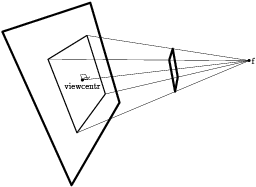
\includegraphics[width=65mm]{thethreekindsofperspec.2} &
        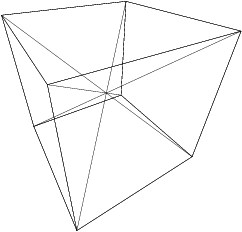
\includegraphics[width=0.25\columnwidth]{cubicfigures.2}
      \end{tabular}
    \end{center}
    \caption{Central projection (default).}
    \label{coniproj}
  \end{figure}
}
\frame{
  \begin{figure}[hbtp]
    \begin{center}
      \begin{tabular}{cc}
        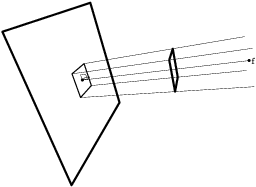
\includegraphics[width=65mm]{thethreekindsofperspec.1} &
        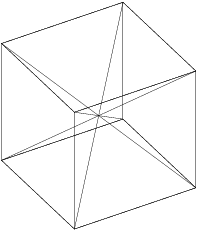
\includegraphics[width=0.25\columnwidth]{cubicfigures.1}
      \end{tabular}
    \end{center}
    \caption{Parallel projection.}
    \label{paraproj}
  \end{figure}
}
\frame{
  \begin{figure}[hbtp]
    \begin{center}
      \begin{tabular}{cc}
        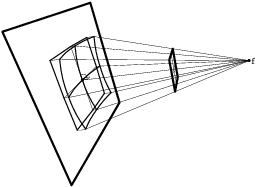
\includegraphics[width=65mm]{thethreekindsofperspec.3} &
        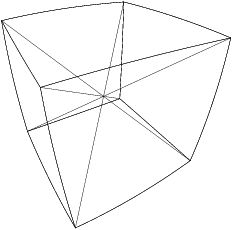
\includegraphics[width=0.25\columnwidth]{cubicfigures.3}
      \end{tabular}
    \end{center}
    \caption{Spherical projection. The
      spherical projection is the composition of two operations: (i)~there
      is a projection onto a sphere and (ii)~the sphere is plaited
      onto the projection plane.}
    \label{spheproj}
  \end{figure}
}

\subsection{Bugs}

\frame{
  \changeableframetitle{Bugs}
  It is important to keep in mind that some capabilities of \FP,
  although usable, may be considered ``buggy'' or only partially
  implemented. These include the drawing of cylinders with holes, as
  in figure \ref{buggydisc}.
}

\frame{
  \begin{figure}[hbtp]
    \begin{center}
      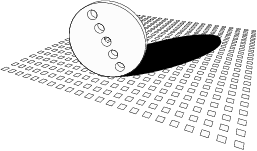
\includegraphics[width=65mm]{fakehole.1}
    \end{center}
    \caption{\FP\ example containing a 
      \myem{rigorousdisc} with five holes, four of which are fake.}
    \label{buggydisc}
  \end{figure}
}

\subsection{Moving on, slowly}

\frame{
  \changeableframetitle{Moving on}
  It is highly beneficial to
  be able to understand and cope with \MP\ error messages as
  \FP\ has no protection against mistaken inputs. One
  probable cause of errors is the use of variables with the name of
  procedures (macros), like
  \begin{quote}
\begin{alltt}
X, Y, Z, W, N, rp, cb, ps, vp
\end{alltt}
  \end{quote}
  All other procedure names have six or more characters.
}

\frame{
  The user must be aware that \MP\ has a limited arithmetic power
  and that the author has limited programming skills,
  which may lead to unperfect 3D figures, very long processing
  time or shear bugs.
  It's advisable not to try very complex diagrams at first 
  and it's recommended to
  keep 3D coordinates near order 1 (default \MP\ units).
}

\frame{
  All three-dimensional \FP\ macros are build apon 
  the \MP\
  \myem{color} variable type. It looks like this:
  \begin{quote}
\begin{alltt}
(red,green,blue)
\end{alltt}
  \end{quote}

  Its components may, nevertheless,
  be arbtitrary numbers, like:
  \begin{quote}
\begin{alltt}
(X,Y,Z)
\end{alltt}
  \end{quote}
  So, the
  \myem{color} type is adequate to define not only colors but
  also 3D points and vectors.
}

\frame{
  \changeableframetitle{Hello world}
  One very minimalistic example program could be:
  \begin{quote}
\begin{alltt}
input featpost3Dplus2D;
beginfig(1);
  cartaxes(1,1,1);
endfig;
end.
\end{alltt}
  \end{quote}
  where \myem{cartaxes} is a
  \FP\ macro that produces
  the Cartesian reference frame with axis labels.
}

\frame{
  The main variable of any three-dimensional figure is the
  point of view. \FP\ uses the variable \myem{f}
  as the point of view. \myem{Spread} is another global
  variable that controls the size of the projection. 
  Therefore the minimalistic program above should also contain, 
  for example:
  \begin{quote}
\begin{alltt}
f:=(6,1,3);
Spread:=40;
\end{alltt}
  \end{quote}
}

\subsection{Why \FP?}

\frame{
  \changeableframetitle{Why \FP?}
  \FP\ is good enough to produce scientific diagrams:
  \begin{itemize}
  \item Figure 1 of 
    \href{http://pre.aps.org/abstract/PRE/v60/i3/p2985_1}{\textit{Phys. Rev. E},
      \textbf{60}, 2985-2989 (1999)}.
  \item Figures 4, 6 and 8 of
    \href{http://www.springerlink.com/content/pmwu8a2y9pkxr5rq/}{\textit{Eur. 
        Phys. J. E}, \textbf{2}, 351-358 (2000)}.
  \item Figures 8 and 12 of
    \href{http://www.springerlink.com/content/w41308176vnk7408/}{\textit{Eur. 
        Phys. J. E}, \textbf{20}, 55-61 (2006)}.
  \end{itemize}
}

\subsection{A small subset of features}

\subsubsection{Angles}

\frame{
  \changeableframetitle{Angles}
  Some problems often require defining angles, and diagrams are
  needed to visualize their meanings.  The \myem{angline} and
  \myem{squareangline} macros support this (see figure \ref{figcartaxes2}).
}

\frame{
  \begin{figure}[hbtp]
    \begin{center}
      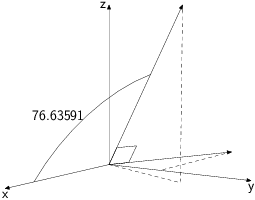
\includegraphics[width=65mm]{cartaxes.2}
    \end{center}
    \caption{Example that uses \myem{cartaxes}, \myem{squareangline},
      \myem{angline} and \myem{getangle}.}
    \label{figcartaxes2}
  \end{figure}
}

\subsubsection{Parametric lines}

\frame{
  \changeableframetitle{Parametric lines}
  Visualizing parametric lines is another need.  When two
  lines cross, one should be able to see which line is in front of the
  other. The macro \myem{emptyline} can help here (see figure
  \ref{induction}).
}

\frame{
  \begin{figure}[hbtp]
    \begin{center}
      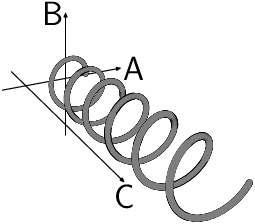
\includegraphics[width=65mm]{parafuso.1}
    \end{center}
    \caption{\FP\ diagram using \myem{emptyline}.}
    \label{induction}
  \end{figure}
}

\subsubsection{Curved solids}

\frame{
  \changeableframetitle{Curved solids}
  \begin{sloppypar}
    Some curved surface solid objects can be drawn with \FP. Among them
    are cones (\myem{very\-good\-cone}), cylinders (\myem{rigorous\-disc})
    and globes (\myem{trop\-ical\-globe}). These can also cast their shadows
    on a horizontal plane (see figure
    \ref{anddisc}). The production of shadows
    involves the global variables \myem{LightSource}, \myem{ShadowOn} 
    and \myem{HoriZon}.
  \end{sloppypar}
}

\frame{
  \begin{figure}[hbtp]
    \begin{center}
      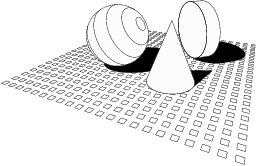
\includegraphics[width=65mm]{stageforthree.3}
    \end{center}
    \caption{\FP\ diagram using
      the macros \myem{rigorousdisc}, \myem{verygoodcone},
      \myem{tropicalglobe} and \myem{setthestage}.}
    \label{anddisc}
  \end{figure}
}

\subsubsection{Fat sticks}

\frame{
  \changeableframetitle{Fat sticks}
  One feature that merges 2D and 3D involves what might be called 
  ``fat sticks''. A fat stick resembles the Teflon magnets used to mix
  chemicals. They have volume but can be drawn like a small straight
  line segment stroked with a big \myem{pencircle}. Fat sticks may be used
  to represent direction fields (unitary vector fields without arrows).
  See figure \ref{nsmetica}.
}

\frame{
  \begin{figure}[hbtp]
    \begin{center}
      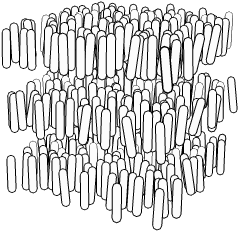
\includegraphics[width=65mm]{nsmetica.1}
    \end{center}
    \caption{\FP\ direction field macro \myem{director\_invisible} was
      used to produce this representation of the molecular structure of
      a Smectic A liquid crystal.}
    \label{nsmetica}
  \end{figure}
}

\subsubsection{From 3D to 2D}

\frame{
  \changeableframetitle{From 3D to 2D}
  The most important macro is \myem{rp} that converts 3D points
  to two-dimensional (2D) rigorous, orthogonal
  or fish-eye projections. To draw a line in
  3D-space try
  \begin{quote}
\begin{alltt}
draw rp(a)--rp(b);
\end{alltt}
  \end{quote}
  where
  \myem{a} and \myem{b} are points in space
  (of \myem{color} type).
}

\frame{
  \changeableframetitle{``Straight lines''}
  But if you're going for fish-eye it's better to
  \begin{quote}
\begin{alltt}
draw pathofstraightline(a,b);
\end{alltt}
  \end{quote}
  If
  you don't know, leave it as
  \begin{quote}
\begin{alltt}
drawsegment(a,b);
\end{alltt}
  \end{quote}
}

\subsubsection{Intersections}

The most advanced feature of \FP\ is the
ability to calculate the intersections of planar and
convex polygons\footnote{Unfortunately, this is also the
most "bugged" feature.}. It can draw the visible
part of arbitrary sets of polygons as in
the following program:
\begin{quote}
\begin{alltt}
input featpost3Dplus2D;
numeric phi;
phi = 0.5*(1+sqrt(5));
V1 := ( 1, phi,0);V2 := (-1, phi,0);
V3 := (-1,-phi,0);V4 := ( 1,-phi,0);
V5 := (0, 1, phi);V6 := (0,-1, phi);
V7 := (0,-1,-phi);V8 := (0, 1,-phi);
V9 := ( phi,0, 1);V10:= ( phi,0,-1);
V11:= (-phi,0,-1);V12:= (-phi,0, 1);
makeface1(1,2,3,4);makeface2(5,6,7,8);
makeface3(9,10,11,12);
beginfig(1);
  sharpraytrace;
endfig;
end
\end{alltt}
\end{quote}
See figure \ref{figsharpraytrace}.

\frame{
  \begin{figure}[bpt]
    \begin{center}
      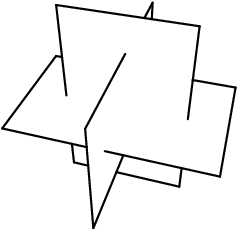
\includegraphics[width=65mm]{sharpraytrace.1}
    \end{center}
    \caption{Intersecting polygons drawn with the macro \myem{sharpraytrace}.}
    \label{figsharpraytrace}
  \end{figure}
}

\subsubsection{Coming back to 3D from 2D}

\frame{
  \changeableframetitle{Coming back to 3D from 2D}
  It is possible to do an "automatic perspective tuning"
  with the aid of macro \myem{photoreverse}. Please, refer both to example
  \myem{photoreverse.mp} (see figure \ref{figphotoreverse}) and to the
  following web page: 
  \href{http://matagalatlante.org/nobre/hyt/technicaldrawfromphoto.html}{FeatPost
    Deeper Technicalities}. 
}

\frame{
  \begin{figure}[bpt]
    \begin{center}
      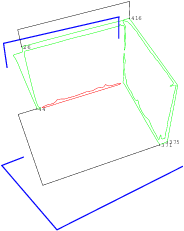
\includegraphics[width=0.45\columnwidth]{photoreverse.1}
    \end{center}
    \caption{Example that uses \myem{photoreverse}. It may
      not work when vertical lines are not vertical in
      average on the photo.}
    \label{figphotoreverse}
  \end{figure}
}

The idea here is to: (i) have a \MP-coded vectorized image; (ii) associate 3D
coordinates to a few specific points of the vectorized image; (iii)
use \myem{photoreverse} to obtain the perspective parameters
corresponding to the image; and (iv) use those perspective parameters to
draw 3D matching schematic diagrams on the image.

\subsubsection{Coming back to 3D from 1D}

\frame{
  \changeableframetitle{Coming back to 3D from 1D}
  Using almost the same algorithm as \myem{photoreverse}, the
  macro \myem{improvertex} allows one to approximate a
  point in 3D-space with given distances $d$ from three other
  points (an initial guess $\vec{i}$ is required).
  \begin{center}
    \myem{point := improvertex}( $\vec{a}$, $d_a$, $\vec{b}$, $d_b$, 
    $\vec{c}$, $d_c$, $\vec{i}$ );
  \end{center}
}

\frame{
  \changeableframetitle{\myem{ultraimprovertex}}
  Approximating a
  point in 3D-space with given distances from three other
  points is the same as calculating the intersection of three spheres.
  And the method to do that is the same as the method to calculate the
  intersection of a plane, a cylinder and a spheroid (see figure
  \ref{figultraimprove}). 
}

\frame{
  \begin{figure}[bpt]
    \begin{center}
      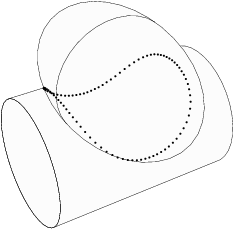
\includegraphics[width=0.45\columnwidth]{ultraimprovertex.1}
    \end{center}
    \caption{Example that uses \myem{ultraimprovertex}.}
    \label{figultraimprove}
  \end{figure}
}

\subsubsection{Scalar function minimization}

\frame{
  \changeableframetitle{Scalar function minimization}
  Macro \myem{minimizestep} is a 
  minimization routine for scalar functions like $y=f(x)$ where an initial
  triplet $(x_1,x_2,x_3)$ with $x_1<x_2<x_3$ is given as a parabolic squeleton that
  provides a way to search for the smallest value of $y$ (if iterated).
  \begin{center}
    \myem{point := minimizestep}( $\vec{x}$ )( $f$ );
  \end{center}
}

\mode<presentation>{\frame{
  \changeableframetitle{The features}
  3D dots, vectors, flat and curved arrows, angles, parametric
  lines, circles and ellipses, cuboids, cones, cylinders, cylindric
  holes, parts of cylindrical surfaces, spheres and spheroids, globes,
  hemispheres, tora, elliptical frusta, revolution paraboloids, 
  polygons, polyhedra, functional and parametric surfaces, direction
  fields, field lines and trajectories in vector fields (differential
  equations), schematic automobiles, schematic electric charges,
  automatic perspective tuning, 2D representation of ropes, reference
  horizontal surfaces, hexagonal plots, schematic 2D springs, zig--zag
  lines, irregular circles, selective intersection of two circles, 2D
  detection of tangency, paths for laser cutting  machines,
  minimization of scalar functions, intersection of 2D areas,
  intersection point of three spheres, intersection point of a plane,
  a cylinder and a spheroid, intersection of a straight line and a
  spheroid, intersection of a straight line and a torus.

  And much more.
}}

\section{Reference Manual}

Some words about notation.
The meaning of macro, function, procedure and routine is the same.
Global variables are presented like this:
\begin{quote}
\begin{alltt}
vartype var, anothervar
anothervartype yetanothervar
\end{alltt}
\end{quote}
Explanation of \myem{var}, \myem{anothervar} and
\myem{yetanothervar}. \myem{vartype} can be any one of
\MP\ types but the meaning
of \myem{color} is a three-dimensional point or vector, not an
actual color like yellow, black or white. If the meaning is
an actual color then the type will be \myem{colour}.
Most of the global variables have default values.

Functions are presented like this:
\begin{itemize}
\item returntype {\bfseries function()}
Explanation of this function. ``returntype'' can be any one of \MP\
types plus global, draw,  drawlabel or MD.
``global'' means that the function
changes some of the global variables. ``draw'' means that
the function
changes the currentpicture. ``drawlabel'' means that the
function changes
the currentpicture and adds text to it. ``MD'' means that the
returntype is the same as the type of the arguments (1, 2, 3 or 4D,
that is \myem{numeric}, \myem{pair}, \myem{color} or \myem{cmykcolor}).
\begin{enumerate}
\item  \myem{type1}
Explanation of the first argument. The type of
one argument can be any one
of \MP\ types plus \myem{suffix} or
\myem{text}.
\item  \myem{type2}
Explanation of the second argument.
There is the possibility that the
function has no arguments. In that case the
function is presented like
"\myem{returntype} {\bfseries function}".
\item  Etc.
\end{enumerate}
\end{itemize}

\subsection{Global variables}

\begin{quote}
\begin{alltt}
boolean ParallelProj
boolean SphericalDistortion
boolean MalcomX
\end{alltt}
\end{quote}
Kind of projection calculated by \myem{rp}.
By default projections
are rigorous but if \myem{ParallelProj} is set
\myem{true} then
parallel lines remain parallel in the projection.
It is the same as
placing the point of view infinitely far without loosing
sight.
If \myem{SphericalDistortion} is set \myem{true}
there will be a
distortion coming from: (i) the projection being done
on a sphere of
center \myem{f} and (ii) this sphere being plaited
onto the paper page.
When \myem{MalcomX} is set \myem{true}, perspectives are calculated
with the x coordinate (first coordinate) replaced by the fourth
coordinate. The idea here is to use the fourth coordinate as ``time''
and visualize yz projections of an animation in a single
figure\footnote{To be developed in future versions.}.   

\frame{
  \begin{figure}[bpt]
    \begin{center}
      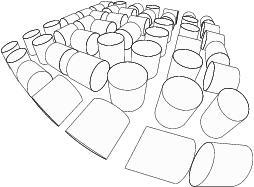
\includegraphics[width=65mm]{rigorousdiscSD.1}
    \end{center}
    \caption{Figure that uses \myem{SphericalDistortion:=true}
      and \myem{rigorousdisc}.}
    \label{sphericaldisc}
  \end{figure}
}

\begin{quote}
\begin{alltt}
color f, viewcentr
\end{alltt}
\end{quote}
The point of view is \myem{f}. The plane or sphere
of projection contains
the center of view \myem{viewcentr}.
The axis, parallel to zz, that contains the
\myem{viewcentr} is projected on a vertical line.
\begin{quote}
\begin{alltt}
numeric MaxFearLimit
\end{alltt}
\end{quote}
The above variable defines the maximum allowed 3D distance between
\myem{viewcentr} and the projection of a point as calculated by
\myem{rp} (remember that 3D distances have no units). Everything
located beyond this maximum is compressed into a circumference.  
\begin{quote}
\begin{alltt}
numeric Spread
pair ShiftV, OriginProjPagePos
numeric PageWidth
numeric PageHeight
\end{alltt}
\end{quote}
These variables control
the placement of the projection on the
paper. \myem{Spread} is the magnification
and \myem{ShiftV} is the position of the
\myem{viewcentr} projection on the
paper. But, if at some point in your program you introduce
\myem{produce\_auto\_scale} then the
\myem{currentpicture} will be
centered at \myem{OriginProjPagePos}
and scaled to fit inside a rectangle of
\myem{PageWidth} by \myem{PageHeight}.
\begin{quote}
\begin{alltt}
color V[]
color L[]p[]
color F[]p[]
\end{alltt}
\end{quote}
Vertexes, lines and faces.
The idea here is to draw
polygons and/or arbitrary lines in 3D space.
Defining the polygons and
the lines can be a bit tedious as \FP\ is not
interactive\footnote{The lines could become the skeleton of NURBS.}. 
First, one defines a list of the
vertexes (\myem{V[]}) that define the
polygons and/or the lines.
There is a list of polygons and a list of
lines. Each polygon (\myem{F[]p[]}) or
line (\myem{L[]p[]}) is itself a list of vertexes.
All vertexes of the same poligon should belong
to the same plane.
\begin{quote}
\begin{alltt}
numeric NL
numeric npl[]
numeric NF
numeric npf[]
\end{alltt}
\end{quote}
Number of lines, number of vertexes of each line,
number of faces, number of vertexes of each face.
\begin{quote}
\begin{alltt}
numeric PrintStep
\end{alltt}
\end{quote}
\myem{Printstep} is the size of iterative jumps
along lines. Used by
\myem{lineraytrace}, \myem{faceraytrace} and
\myem{pathofstraightline}.
Big \myem{Printstep}s make fast \myem{lineraytrace}ings.
\begin{quote}
\begin{alltt}
boolean FCD[]
colour TableC[]
numeric TableColors
numeric FC[]
colour HigColor
colour SubColor
color LightSource
\end{alltt}
\end{quote}
\myem{FCD} means "face color defined". The
\myem{draw\_invisible} macro draws
polygons in colour, if it is defined. The colour must be
selected from the table of colours \myem{TableC} that has
as many as \myem{TableColors}. The colour \myem{FC}
of each polygon will depend on its position relatively to
\myem{LightSource} where we suppose there is a lamp that
emits light coloured \myem{HigColor}. Furthermore the
colour of each polygon may be modified if it belongs to a
functional or parametric surface. In this case, if we are
looking at the polygon from below than \myem{SubColor} is
subtracted from its colour.
\begin{quote}
\begin{alltt}
numeric RopeColorSeq[]
numeric RopeColors
\end{alltt}
\end{quote}
The above variables are used by \myem{ropepattern}.

\begin{quote}
\begin{alltt}
numeric TDAtiplen
numeric TDAhalftipbase
numeric TDAhalfthick
\end{alltt}
\end{quote}
The above variables control the shape of Three-Dimensional Arrows.

\begin{quote}
\begin{alltt}
boolean ShadowOn
numeric HoriZon
\end{alltt}
\end{quote}
When \myem{ShadowOn} is set \myem{true}, some objects can
cast a black shadow on a horizontal plane of \myem{Z}
coordinate equal to \myem{HoriZon} (an area from
this plane may be drawn with \myem{setthestage} or with
\myem{setthearena}) as if there is a punctual source of light at
\myem{LightSource}.
The macros that can produce shadows, in addition to their
specific production, are
\begin{itemize}
\item \myem{emptyline}
\item \myem{rigorousdisc}
\item \myem{verygoodcone}
\item \myem{tropicalglobe}
\item \myem{positivecharge}
\item \myem{whatisthis}
\item \myem{spheroid}
\item \myem{ellipsoid}
\item \myem{kindofcube}
\item \myem{draw\_all\_test}
\item \myem{fill\_faces}
\item \myem{smoothtorus}
\end{itemize}
All macros that contain {\bfseries shadow} in their name
calculate the location of shadows using \myem{cb}. These are:
\myem{circleshadowpath};
\myem{signalshadowvertex};
\myem{ellipticshadowpath};
\myem{circleshadowpath};
\myem{spheroidshadow};
\myem{ellipsoidshadow};
\myem{torushadow};
\myem{rigorousfearshadowpath}; and
\myem{faceshadowpath}.
\begin{quote}
\begin{alltt}
path VGAborder
\end{alltt}
\end{quote}
This path and the macro \myem{produce\_vga\_border} are
meant to help you clip the \myem{currentpicture} to a 4:3
rectangle as in a (old) movie frame.

\begin{quote}
\begin{alltt}
pair PhotoPair[]
color PhotoPoint[]
numeric PhotoMarks
\end{alltt}
\end{quote}
The above variables are used by \myem{photoreverse}.

\begin{quote}
\begin{alltt}
pen ForePen, BackPen
path CLPath
numeric NCL
\end{alltt}
\end{quote}
The above variables are used by \myem{closedline}.

\begin{quote}
\begin{alltt}
boolean OverRidePolyhedricColor
string ostr[]
numeric ActuC, Nobjects, RefDist[]
\end{alltt}
\end{quote}
\myem{OverRidePolyhedricColor} is used by \myem{fillfacewithlight}.
\myem{Nobjects}, \myem{ostr} and \myem{RefDist[]} are auxiliary
variables used by \myem{getready} and \myem{doitnow}.
\myem{Actuc} is used both by \myem{hexagonaltrimesh} and
by \myem{partrimesh}.

\subsection{Definitions}

\begin{itemize}
\item global makeline@\#( text1)
\item global makeface@\#( text1)
\end{itemize}
Both of these functions ease the task of
defining lines and polygons. Just
provide a list of vertexes in a correct
sequence for each polygon and/or
line. Suppose a tetrahedron
\begin{quote}
\begin{alltt}
V3:=(+1,-1,-1);V2:=(-1,+1,-1);
V4:=(+1,+1,+1);V1:=(-1,-1,+1);
makeface2(1,2,3);makeface3(1,2,4);
makeface1(3,4,1);makeface4(3,4,2);
\end{alltt}
\end{quote}
The
number in the last makeface or last
makeline procedure name must be the
number of polygons or lines. All polygons and lines from 1 upto this
number must be defined but the sorting may be any of your liking.

\subsection{Macros}

\subsubsection{Very Basic Macros}

\begin{itemize}
\item numeric {\bfseries X()}
Returns the first coordinate of a point or vector (triplet of
color type) if \myem{MalcomX} is false but returns the fourth coordinate
of a tetraplet (of cmykcolor type) if \myem{MalcomX} is true. 
\item numeric {\bfseries Y()}
Returns the second coordinate of a point or vector.
Replaces \myem{greenpart}.
\item numeric {\bfseries Z()}
Returns the third coordinate of a point or vector.
Replaces \myem{bluepart}.
\item numeric {\bfseries W()}
Returns the fourth coordinate of a 4D point or vector.
Replaces \myem{blackpart}.
\item cmykcolor {\bfseries makecmyk()} Produces a tetraplet from a
  triplet and a scalar.
\item color {\bfseries maketrio()} This is, in fact, a projection from
  4D into 3D. The single input is a tetraplet and the output is a
  triplet (the fourth coordinate is discarded). The output triplet
  takes in consideration the value of \myem{MalcomX} (see \myem{X}). 
\item draw {\bfseries produce\_auto\_scale}
The currentpicture is centered in, and adjusted
to the size of, an A4
paper page. This avoids the control of \myem{Spread} and
\myem{ShiftV}.
\item string {\bfseries cstr()} Converts a color into its
string. Usefull in combination with \myem{getready}.
\item string {\bfseries bstr()} Converts a boolean 
expression into its
string. Usefull in combination with \myem{getready}.
\end{itemize}

\subsubsection{Vector Calculus}

\begin{itemize}
\item color {\bfseries N()} Unit vector. Returns
\myem{black} (the null vector) when the argument has
null norm. The "N" means "normalized".
\item numeric {\bfseries cdotprod()} Dot product of two
vectors.
\item color {\bfseries ccrossprod()} Cross product of two
vectors.
\item numeric {\bfseries ndotprod()} Cossine of the angle
beetween two vectors.
\item color {\bfseries ncrossprod()} Normalized cross product
of twovectors.
\item numeric {\bfseries conorm()} Euclidean norm of a
vector.
\item numeric {\bfseries cmyknorm()} Euclidean norm of a
4D vector. Should not be used when \myem{MalcomX} is \myem{true}.
\item numeric {\bfseries getangle()} Angle beetween two
vectors.
\item numeric {\bfseries getcossine()} Cossine of the angle between
  segment A and segment B, where A connects \myem{f} and the center of
  a sphere, and where B contains \myem{f} and is tangent to that sphere.
\item pair {\bfseries getanglepair()} Orientation angles
of a vector. The first angle (\myem{xpart}) is
measured beetween the vector projection on the \myem{XY}
plane and the \myem{X} axis. The second angle
(\myem{ypart}) is measured
beetween the vector and its projection on the \myem{XY}
plane. This may be usefull to find the arguments of
\myem{kindofcube}
\item color {\bfseries eulerrotation()} Three-dimensional
rotation of a vector. See the figure \ref{kindofcube2} to visualize
the following movement: (i) grab the \myem{X} component of the
vector; (ii) rotate it on the \myem{XY} plane as
much as the first argument; 
(iii) raise it up as much as the second argument; and
(iv) turn it around as much as the third argument.
\begin{enumerate}
\item \myem{numeric} Angle of rotation around the
\myem{Z} component.
\item \myem{numeric} Angle of rotation around the
rotated \myem{Y} component.
\item \myem{numeric} Angle of rotation around the
two times rotated \myem{X} component.
\item \myem{color} Vector to be rotated.
\end{enumerate}
\item color {\bfseries randomfear} Generates a randomly
oriented unit vector.
\item MD {\bfseries planarrotation($\vec{A},\vec{B},\theta$)} $=\vec{A}\cos\theta+\vec{B}\sin\theta$
\item color {\bfseries rotvecaroundanother} Rotates a vector around
  another.
\begin{enumerate}
\item \myem{numeric} Angle of rotation around the fixed vector.
\item \myem{color} Vector to be rotated.
\item \myem{color} Fixed vector.
\end{enumerate}

\end{itemize}



\subsubsection{Projection Macros}

\begin{itemize}
\item pair {\bfseries rp()} Converts spatial positions into
planar positions on the paper page. The conversion
considers the values of the following global
variables: \myem{viewcentr},
\myem{ParallelProj}, \myem{SphericalDistortion},
\myem{Spread}, \myem{ShiftV} and \myem{MaxFearLimit}. When both
\myem{ParallelProj} and \myem{SphericalDistortion}
are \myem{false} it won't work if either (i) the
vectors \myem{f-viewcentr} and \myem{f-R} are
perpendicular (\myem{R} is the argument) or (ii)
\myem{f} and \myem{viewcentr} share the same
\myem{X} and \myem{Y} coordinates. 
\begin{enumerate}
\item \myem{color} Spatial position.
\end{enumerate}
\item pair {\bfseries vp()} Converts spatial directions into
planar positions on the paper page. These positions are the
vanishing points of those directions. The conversion
considers the values of the same global
variables as \myem{rp}.
\begin{enumerate}
\item \myem{color} Spatial direction.
\end{enumerate}
\item color {\bfseries cb()} Calculates the position of the
shadow of a point. Uses \myem{HoriZon} and
\myem{LightSource}.
\begin{enumerate}
\item \myem{color} Point position.
\end{enumerate}
\item color {\bfseries projectpoint()} Calculates the
intersection beetween a plane and a straight
line. The plane contains a given point and is
perpendicular to the line connecting the
\myem{LightSource} and this same point.
The line is defined by another given point and the
\myem{LightSource}. Summary: \myem{projectpoint}
returns the projection of the second argument on a
plane that contains the first argument. Can be used to
draw shadows cast on generic planes.
\begin{enumerate}
\item \myem{color} Origin of the projection plane.
\item \myem{color} Point to be projected.
\end{enumerate}
\item color {\bfseries lineintersectplan()} Calculates the
intersection beetween a generic plane and a straight
line. The plane contains a given point and is
perpendicular to a given vector.
The line contains a given point and is parallel to 
a given vector. 
\begin{enumerate}
\item \myem{color} Point of the line.
\item \myem{color} Vector parallel to the line.
\item \myem{color} Point of the projection plane.
\item \myem{color} Vector perpendicular to the 
projection plane.
\end{enumerate}
\item numeric {\bfseries ps()} Used by \myem{signalvertex}.
\end{itemize}


\subsubsection{Plain Basic Macros}

\begin{itemize}
\item draw {\bfseries signalvertex()} Draws a dot
sized inversely proportional to its distance from
the viewpoint \myem{f}.
\begin{enumerate}
\item \myem{color} Location.
\item \myem{numeric} Factor of proportionality
("size of the dot").
\item \myem{colour} Colour of the dot.
\end{enumerate}

\frame{
  \begin{figure}[bpt]
    \begin{center}
      
\includegraphics[width=65mm]{torus.1}
    \end{center}
    \caption{Figure that uses \myem{signalvertex}.}
  \end{figure}
}
\item path {\bfseries pathofstraightline()} When using
\myem{SphericalDistortion:=true}, straight lines
look like curves. This macro returns the curved path
of a straight line beetween two points. This path will
have a greater \myem{length} ("time") when
\myem{PrintStep} is made smaller.
\item draw {\bfseries drawsegment()} Alternative 
\myem{pathofstraightline} that avoids the
calculation of all the intermediate points when 
\myem{SphericalDistortion:=false}.
\item drawlabel {\bfseries cartaxes()}
Cartesean axis with prescribed lenghtes and apropriate labels.
\begin{enumerate}
\item \myem{numeric} Length of the \myem{X} axis.
\item \myem{numeric} Length of the \myem{Y} axis.
\item \myem{numeric} Length of the \myem{Z} axis.
\end{enumerate}
\item drawlabel {\bfseries orthaxes()}
Cartesean axis with prescribed lenghtes and prescribed labels.
\begin{enumerate}
\item \myem{numeric} Length of the \myem{X} axis.
\item \myem{label} Label of the \myem{X} axis.
\item \myem{numeric} Length of the \myem{Y} axis.
\item \myem{label} Label of the \myem{Y} axis.
\item \myem{numeric} Length of the \myem{Z} axis.
\item \myem{label} Label of the \myem{Z} axis.
\end{enumerate}
\item draw {\bfseries emptyline()} This procedure produces
a sort of a tube that can cross over itself. It
facilitates the drawing of, for instance, thick
helical curves but it won't
look right if the curves are drawn getting apart from
the point of view. Please, accept this inconveniance.
As like many other \FP\ macros this one
can produce visually correct diagrams only in limited
conditions. Can cast a shadow.
\begin{enumerate}
\item \myem{boolean} Choose \myem{true} to join
this line with a previously drawn line.
\item \myem{numeric} Factor of proportionality
("diameter of the tube"). The tubes are just
sequences of dots drawn by \myem{signalvertex}.
\item \myem{colour} Colour of the tube border.
\item \myem{colour} Colour of the tube.
\item \myem{numeric} Total number of dots on the
tube line.
\item \myem{numeric} Fraction of the tube diameter
that is drawn with the tube colour.
\item \myem{numeric} This is the number of dots
that are redrawn with the colour of the tube for
each drawn dot with the color of the tube
border. Usually 1 or 2 are enough.
\item \myem{text} This is the name a function
that returns a 3D point of the line for each value
of a parameter in beetween 0 and 1.
\end{enumerate}

\frame{
  \begin{figure}[bpt]
    \begin{center}
      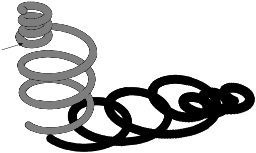
\includegraphics[width=65mm]{joinedemptylines.1}
    \end{center}
    \caption{Figure that uses \myem{emptyline}.
      The junction point of two different lines is indicated
      by an arrow. }
    \label{joinedemptylines}
  \end{figure}
}
\item draw {\bfseries closedline()} This procedure produces
a tube that can cross over itself. It
facilitates the drawing of, for instance, thick
helical curves but it won't
look right as its thickness does not change with the
distance from the point of view. The drawing is
entirely done in two dimensions, so the tube diameter
depends on the global variables \myem{ForePen} and
\myem{BackPen}. There can be more than one
line in a figure but all get the same diameter.
When calling \myem{closedline()} in different
figures of the same program you must reinitialize both
\myem{NCL} and \myem{Nobjects} (because
\myem{closedline()} uses \myem{getready()}).
\begin{enumerate}
\item \myem{boolean} Value of "the line is closed".
\item \myem{numeric} Total number of path segments
on the tube line.
\item \myem{numeric} Use 0.5 or more.
\item \myem{numeric} Use 0.75 or more.
\item \myem{text} This is the name of a function
that returns a 3D point of the line for each value
of a parameter in beetween 0 and 1.
\end{enumerate}
\item drawlabel {\bfseries angline()}
Draws an arch beetween two straight lines with a
common point and places a label
near the middle of the arch (marks an
angle). Note that the arch is not circular. 
\begin{enumerate}
\item \myem{color} Point of one line.
\item \myem{color} Point ot the other line.
\item \myem{color} Common point.
\item \myem{numeric} Distance beetween the arch and
the common point.
\item \myem{picture} Label.
\item \myem{suffix} Position of the label relatively
to the middle of the arch. May
be one of \myem{lft, rt, top, bot, ulft, urt,
llft} and \myem{lrt}.
\end{enumerate}
\item drawlabel {\bfseries anglinen()}
The same as the previous function but the
sixth argument is numeric:
0=\myem{rt};
1=\myem{urt};
2=\myem{top};
3=\myem{ulft};
4=\myem{lft};
5=\myem{llft};
6=\myem{bot};
7=\myem{lrt};
any other number places the label
on the middle of the arch.
\item draw {\bfseries squareangline()}
This is supposed to mark 90 degree angles
but works for any angle value.
\begin{enumerate}
\item \myem{color} Point of one line.
\item \myem{color} Point ot the other line.
\item \myem{color} Common point.
\item \myem{numeric} Distance beetween the "arch"
and the common point.
\end{enumerate}
\item path {\bfseries rigorouscircle()}
3D circle. The total "time" of this path is 8. This
small number makes it easy to select parts of the
path. The circle is drawn using the
"left-hand-rule". If you put your left-hand thumb
parallel the circle axis then the other left-hand
fingers curl in the same sense as the circle
path. This path allways starts, approching the view
point, from a point on a diameter of the
circle that projects orthogonaly to its axis, and
rotating around the axis in the way of the left-hand-rule.
\begin{enumerate}
\item \myem{color} Center of the circle.
\item \myem{color} Direction orthogonal to the
circle (circle axis).
\item \myem{numeric} Radius of the circle.
\end{enumerate}
\frame{
  \begin{figure}[bpt]
    \begin{center}
      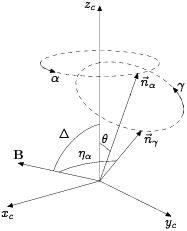
\includegraphics[width=0.45\columnwidth]{anglinerigorouscircle.1}
    \end{center}
    \caption{Figure that uses \myem{anglinen}
      and \myem{rigorouscircle}.}
  \end{figure}
}
\item draw {\bfseries tdarrow()} Draws a flat arrow that
begins at the first argument and ends at the second.
The shape of the arrow is controled by the global
variables \myem{TDAtiplen, TDAhalftipbase, TDAhalfthick}.
This arrow is drawn on the plane that maximizes the perspective of its
width. Also, the tip is contracted when \myem{TDAtiplen} is larger
than the length of the arrow.
\item draw {\bfseries tdcircarrow()} Draws a flat curving arrow. The
  curve is a circular arch on a plane.
The shape of the arrow is controled both by the global
variables \myem{TDAtiplen, TDAhalftipbase, TDAhalfthick} and by the
three last arguments. 
\begin{enumerate}
\item \myem{color} Position of the center ($\vec{c}$).
\item \myem{color} Vector perpendicular to the plane $P$ that contains the
  arrow (rotation axis $\vec{A}$).
\item \myem{numeric} Curve ray.
\item \myem{numeric} Arrow starting angle. Note that the angle is measured
      relative to the axis pointing from $\vec{c}$ to \myem{f} and
      projected onto $P$ ($\vec{B}$). The angle is positive when it
      approaches $\vec{A}\times\vec{B}$. 
\item \myem{numeric} Angular amplitude of the curve (may be negative).
\end{enumerate}
\frame{
  \begin{figure}[bpt]
    \begin{center}
      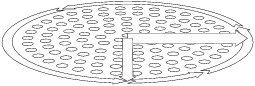
\includegraphics[width=0.45\columnwidth]{tdcircarrow.1}
    \end{center}
    \caption{Figure that uses \myem{tdarrow}
      and \myem{tdcircarrow}.}
  \end{figure}
}
\item path {\bfseries twocyclestogether()} This macro
allows you to draw any solid that has no vertexes
and that has two, exactly two, planar cyclic edges.
In fact, it doesn't need to be a solid. Just
provide the pathes of both cyclic edges as arguments
but note that the returned path is polygonal.
In order to complete
the drawing of this solid you have to choose one of
the edges to be drawn immediatly afterwards. This is
done automatically by the \myem{whatisthis} macro
for the case of two parallel and concentric ellipses.
\item path {\bfseries ellipticpath()} Produces an elliptic
path in 3D space.
\begin{enumerate}
\item \myem{color} Position of the center.
\item \myem{color} Major or minor axis.
\item \myem{color} The other axis.
\end{enumerate}
\item drawlabel {\bfseries labelinspace()} Draw some 2D
\myem{picture} on some 3D plane (only when
\myem{ParallelProj:=true}). Just \myem{Transform}s the
  label in the same
  way as its bounding box, that is, the same way as two perpendicular sides
  of its bounding box. This is only exact for parallel perspectives.
\begin{enumerate}
\item \myem{color} Position for the lower-left
corner. 
\item \myem{color} Orientation of the picture's
bottom edge.
\item \myem{color} Orientation of the picture's
letf edge.
\item \myem{text} 2D picture's name.
\end{enumerate}

\frame{
  \begin{figure}[bpt]
    \begin{center}
      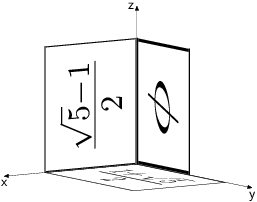
\includegraphics[width=65mm]{labelinspace.1}
    \end{center}
    \caption{Example that uses \myem{labelinspace}.}
  \end{figure}
}
\end{itemize}


\subsubsection{Standard Objects}

\begin{itemize}
\item path {\bfseries goodcirclepath()}
Another 3D circle macro. More rigorous
than \myem{rigorouscircle} but when
the direction ortogonal to the circle is almost
orthogonal to the line \myem{viewpoint--center}
it doesn't work correctly.
The total "time" of this path is 36.
\begin{enumerate}
\item \myem{color} Center of the circle.
\item \myem{color} Direction ortogonal to
the circle.
\item \myem{numeric} Radius of the
circle.
\end{enumerate}
\item draw {\bfseries spatialhalfsfear()} An
hemisphere. Doesn't work with \myem{f} inside it.
\begin{enumerate}
\item \myem{color} Center.
\item \myem{color} Vector ortogonal to
the frontier circle and pointing
out of the concavity.
\item \myem{numeric} Radius of the
(hemi)sphere.
\end{enumerate}
\item path {\bfseries spatialhalfcircle()}
And yet another 3D circle macro. Only the visible or the hidden
part. This is usefull to mark sections of
cylinders or spherical major circles.
\begin{enumerate}
\item \myem{color} Center of the circle.
\item \myem{color} Direction ortogonal to the
circle.
\item \myem{numeric} Radius of the circle.
\item \myem{boolean} The visible part is selected with
\myem{true} and the hidden
with \myem{false}.
\end{enumerate}
\item draw {\bfseries rigorousdisc()}
3D opaque cylinder with/without a hole. Can cast a
shadow (without the hole).
\begin{enumerate}
\item \myem{numeric} Ray of an axial hole.
\item \myem{boolean} Option for completly opaque cylinder
(\myem{true}) or partial
pipe (\myem{false}) when there is no hole. When
the cylinder has an hole this option should be
\myem{true}.
\item \myem{color} Center of one circular base.
\item \myem{numeric} Radius of both circular bases.
\item \myem{color} Vector that defines the length and
orientation of the
cylinder. The addition the third and fifth
arguments should give the
position of the center of the other circular base.
\end{enumerate}
\item draw {\bfseries verygoodcone()} 3D cone. Can cast a shadow.
\begin{enumerate}
\item \myem{bolean} Option to draw dashed evenly
the invisible edge (\myem{true}) or not
(\myem{false}).
\item \myem{color} Center of the circular base.
\item \myem{color} Direction ortogonal to the
circular base.
\item \myem{numeric} Radius of the circular base.
\item \myem{color} Position of the vertex
\end{enumerate}
\item path {\bfseries rigorousfearpath()}
3D sphere. Simple but hard.
\begin{enumerate}
\item \myem{color} Center position.
\item \myem{numeric} Radius.
\end{enumerate}
\item draw {\bfseries tropicalglobe()} Globe with
minor circles. Can cast a shadow.
\begin{enumerate}
\item \myem{numeric} Number of marked latitudes.
\item \myem{color} Center position.
\item \myem{numeric} Radius
\item \myem{color} Axis orientation.
\end{enumerate}
\frame{
  \begin{figure}[bpt]
    \begin{center}
      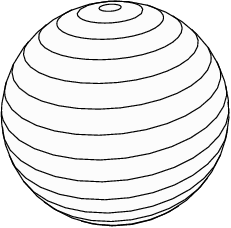
\includegraphics[width=65mm]{tropicalglobe.1}
    \end{center}
    \caption{Figure that uses \myem{tropicalglobe}.}
  \end{figure}
}
\item draw {\bfseries spheroid()} Revolution ellipsoid. Can cast a shadow.
\begin{enumerate}
\item \myem{color} Center position.
\item \myem{color} Position of one pole relative to the center.
\item \myem{numeric} Radius
\end{enumerate}
\frame{
  \begin{figure}[bpt]
    \begin{center}
      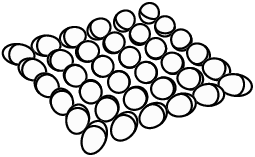
\includegraphics[width=65mm]{revolipsoid.2}
    \end{center}
    \caption{Figure that uses \myem{spheroid}.}
  \end{figure}
}
\item draw {\bfseries whatisthis()} An elliptic
frustum. Both edges are elliptic an have the same
orientation but one may be greater than the other.
Can cast a shadow.
\begin{enumerate}
\item \myem{color} Reference edge center.
\item \myem{color} Major or minor axis.
\item \myem{color} The other axis.
\item \myem{numeric} Length of the original
cylinder.
\item \myem{numeric} Edges axis length ratio.
\end{enumerate}
\item draw {\bfseries kindofcube()} Polyhedron with six
orthogonal faces (cuboid).
\begin{enumerate}
\item \myem{boolean} Also draw the invisible edges
\myem{dashed evenly} (\myem{true}) or do not.
\item \myem{boolean} The reference point may be a
vertex (\myem{true}) or the center(\myem{false}).
\item \myem{color} Reference point.
\item \myem{numeric} Alpha1.
\item \myem{numeric} Alpha2.
\item \myem{numeric} Alpha3.
\item \myem{numeric} L1. Length of the first side.
\item \myem{numeric} L2. Length of the second side.
\item \myem{numeric} L3. Length of the third side.
\end{enumerate}
These arguments are represented in figure \ref{kindofcube2}.

\frame{
  \begin{figure}[bpt]
    \begin{center}
      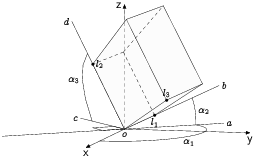
\includegraphics[width=65mm]{kindofcube.2}
    \end{center}
    \caption{Figure that uses and explains
      \myem{kindofcube}. Note that the three indicated
      angles may be used as arguments of \myem{eulerrotation}.}
    \label{kindofcube2}
  \end{figure}
}
\item draw {\bfseries setthestage()} Produces an horizontal
square made of squares. Its \myem{Z} coordinate is defined by
\myem{HoriZon}.
\begin{enumerate}
\item \myem{numeric} Number of squares in each side.
\item \myem{numeric} Size of each side.
\end{enumerate}
\item draw {\bfseries setthearena()} Produces an horizontal
circle made of circles. Its \myem{Z} coordinate is defined by
\myem{HoriZon}. Due to the fact that the center of a
circle is not on the center of its central perspective
projection, this may look a bit strange.
\begin{enumerate}
\item \myem{numeric} Number of circles on a
diameter.
\item \myem{numeric} Diameter.
\end{enumerate}
\item draw {\bfseries smoothtorus()} Toxic donut (not to be
eaten). Produces an error message when \myem{f} is
close to the table. Can cast a shadow.
\begin{enumerate}
\item \myem{color} Center.
\item \myem{color} Direction orthogonal to the
torus plane.
\item \myem{numeric} Big ray.
\item \myem{numeric} Small ray.
\end{enumerate}
\end{itemize}


\subsubsection{Composed Objects}

\begin{itemize}
\item draw {\bfseries positivecharge()} Draws a sphere with a
plus or minus sign on the surface. The horizontal
segment of the sign is drawn on the horizontal plane
that contains the sphere center. The middle point of
this segment is on a vertical plane containing the
viewpoint.
\begin{enumerate}
\item \myem{boolean} Selects the sign (\myem{true}
means positive).
\item \myem{color} Position of the center.
\item \myem{numeric} Sphere ray.
\end{enumerate}

\frame{
  \begin{figure}[bpt]
    \begin{center}
      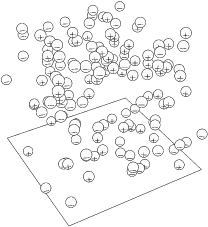
\includegraphics[width=0.55\columnwidth]{positivecharge.1}
    \end{center}
    \caption{Figure that uses \myem{positivecharge},
      \myem{getready} and \myem{doitnow}.}
  \end{figure}
}
\item draw {\bfseries simplecar()} Draws a cuboid and four
discs in a configuration ressembling an automobile. The
first three arguments of \myem{simplecar} are the same
as the the last seven arguments of \myem{kindofcube}
but grouped in colors.
\begin{enumerate}
\item \myem{color} Center of the cuboid that
constitutes the body of the car..
\item \myem{color} Angles defining the orientation
of the car (see \myem{kindofcube}).
\item \myem{color} Dimensions of the car.
\item \myem{color} Characteristics of the front
wheels. \myem{redpart}-distance from the
front. \myem{greenpart}-width of the front wheels (length
of the cylinders). \myem{bluepart}-wheel ray.
\item \myem{color} Same as above for the rear wheels
\end{enumerate}

\frame{
  \begin{figure}[bpt]
    \begin{center}
      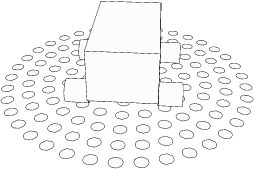
\includegraphics[width=65mm]{simplecar.1}
    \end{center}
    \caption{Figure that uses \myem{setthearena} and
      \myem{simplecar}.}
  \end{figure}
}

\item draw {\bfseries banana()} Draws a cylindrical strip with a mark in
  the middle angle.
  \begin{enumerate}
  \item \myem{color} Center of the base circle.
  \item \myem{numeric} Radius.
  \item \myem{color} Euler angles for the orientation of the strip
    (uses \myem{eulerrotation} as if the cylindrical strip axis is the rotation
    of $\hat{z}$).
  \item \myem{numeric} Length of the cylindrical strip.
  \item \myem{numeric} Angular amplitude of half of the cylindrical strip.
  \end{enumerate}
\frame{
  \begin{figure}[bpt]
    \begin{center}
      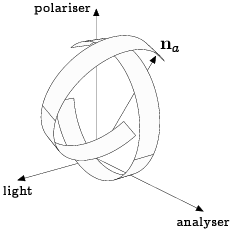
\includegraphics[width=65mm]{bananadimmer.1}
    \end{center}
    \caption{Figure that uses \myem{banana}.}
  \end{figure}
}

\item draw {\bfseries quartertorus()} Draws a part of a torus.
  \begin{enumerate}
  \item \myem{color} Center of the base torus.
  \item \myem{color} Vector indicating the position, relative to the
    center of the base torus, of the center of the circle obtained by
    cutting the base torus through a plane containing its axle. 
  \item \myem{color} Vector indicating the orientation of another
    similar cutting plane (the norm of vector has no meaning).
  \item \myem{numeric} Radius of cross-section circles.
  \end{enumerate}
\frame{
  \begin{figure}[bpt]
    \begin{center}
      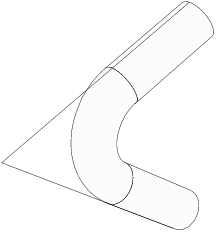
\includegraphics[width=65mm]{quartertorus.2}
    \end{center}
    \caption{Figure that uses \myem{quartertorus}.}
  \end{figure}
}

\end{itemize}


\subsubsection{Shadow Pathes}

Please remember that not all shadows are pathes. 
\begin{itemize}
\item draw {\bfseries signalshadowvertex()} Draws the
shadow of a \myem{signalvertex} dot. Used by \myem{emptyline}.
\begin{enumerate}
\item \myem{color} Location of the light-blocking dot.
\item \myem{numeric} Factor of proportionality
("size of the dot").
\item \myem{colour} Colour of the dot.
\end{enumerate}
\item path {\bfseries ellipticshadowpath()} Produces the
shadow of an elliptic path.
\begin{enumerate}
\item \myem{color} Position of the center.
\item \myem{color} Major or minor axis.
\item \myem{color} The other axis.
\end{enumerate}
\item path {\bfseries circleshadowpath()} Produces the
shadow of a circle.
\begin{enumerate}
\item \myem{color} Center of the circle.
\item \myem{color} Direction ortogonal to
the circle.
\item \myem{numeric} Radius of the
circle.
\end{enumerate}
\item path {\bfseries rigorousfearshadowpath()}
3D sphere shadow.
\begin{enumerate}
\item \myem{color} Center position.
\item \myem{numeric} Radius.
\end{enumerate}
\end{itemize}


\subsubsection{Differential Equations}

Before we proceed, be aware that solving differential
equations (DE) is mainly an experimental activity. The most
probable result of a procedure that atempts to solve a DE
is garbage. The procedure may be unstable, the solution
may be littered with singularities or something may go
wrong. If you don't have a basic understanding of
differential equations then skip this section, please.

\begin{itemize}
\item path {\bfseries fieldlinepath()} A vectorial field line is
everywhere tangent to the field vectors.
Two different parallel fields
have the same field lines. So the field only
constrains the direction of the field lines, not any kind
of "speed" and, therefore, it is recommended to
normalize the field before using this macro that
contains a second-order Runge-Kutta method
implementation.
\begin{enumerate}
\item \myem{numeric} Total number of steps.
\item \myem{color} Initial position.
\item \myem{numeric} Step (arc)length.
\item \myem{text} Name of the function that
returns a field vector for each 3D position.
\end{enumerate}
\item path {\bfseries trajectorypath()} The acceleration of a
particle in a conservative force field is equal to the
ratio (conservative force)/(particle mass). The
acceleration is also equal to the second order time
derivative of the particle position. This produces a
second order differential equation that we solve using a
second-order Runge-Kutta method implementation.
\begin{enumerate}
\item \myem{numeric} Total number of steps.
\item \myem{color} Initial position.
\item \myem{color} Initial velocity.
\item \myem{numeric} Time step.
\item \myem{text} Name of the function that
returns a (force/mass) vector for each 3D position.
\end{enumerate}
\item path {\bfseries magnetictrajectorypath()} The
acceleration of a
charged particle in a magnetic field is equal to the
ratio (magnetic force)/(particle mass) but the magnetic
force depends on both the velocity and the magnetic field. The
acceleration is also equal to the second order time
derivative of the particle position. This produces a
second order differential equation that we solve using a
fourth-order Runge-Kutta method implementation.
\begin{enumerate}
\item \myem{numeric} Total number of steps.
\item \myem{color} Initial position.
\item \myem{color} Initial velocity.
\item \myem{numeric} Time step.
\item \myem{text} Name of the function that
returns a (charge)*(magnetic field)/(partcle mass)
vector for each 3D position.
\end{enumerate}
\end{itemize}

\subsubsection{Renderers}

\begin{itemize}
\item draw {\bfseries sharpraytrace} Heavy procedure that
draws only the visible part of all edges of all defined
faces. There's no point in using this procedure when
there are no intersections beetween faces. Any how
this will not work for non-convex faces nor when
\myem{SphericalDistortion:=true}.
\item draw {\bfseries lineraytrace()} Draws only the
visible part of all defined lines using sequences of dots
(\myem{signalvertex} and \myem{PrintStep}).
\begin{enumerate}
\item \myem{numeric} Dot size.
\item \myem{colour} Dot colour.
\end{enumerate}
\item draw {\bfseries faceraytrace()} Draws only the
visible part of all edges of all defined faces
using sequences of dots
(\myem{signalvertex} and \myem{PrintStep}).
\begin{enumerate}
\item \myem{numeric} Dot size.
\item \myem{colour} Dot colour.
\end{enumerate}
\item draw {\bfseries draw\_all\_test()} Draws all defined
edges (and lines) in a correct way independently of
the kind of projection used. Can cast a shadow (but
the shadow is not correct when
\myem{SphericalDistortion:=true}).
\begin{enumerate}
\item \myem{boolean} If \myem{true} the lines
are also drawn.
\end{enumerate}
\item draw {\bfseries fill\_faces()} Unfills and draws all
faces in the order they were defined (without
sorting). Can cast a shadow.
\begin{enumerate}
\item \myem{text} Like the argument of
\myem{drawoptions} but used only inside this
macro and only for the edges.
\end{enumerate}
\item draw {\bfseries draw\_invisible()} This is a fast way
of removing hidden lines that doesn't
allow for intersecting polygons nor
polygons of very different area. It works by
+sorting all polygons by
distance to \myem{f} and then by "filling" the
polygons. This routine may be used to draw graphs
of 3D surfaces.
\begin{enumerate}
\item \myem{boolean} If \myem{true} polygons are
sorted relatively to
nearest vertex and, if \myem{false}, relatively to their
mass center. Choose \myem{false} for surface
plots.
\item \myem{boolean} If \myem{false} then the
polygons are painted with their \myem{FC} colour
modified by \myem{LightSource}. If \myem{true}
then the next two arguments are used and the
polygons are darkened proportionaly to their
distance from \myem{f}.
\item \myem{colour} Colour of faces.
\item \myem{colour} Colour of the edges.
\end{enumerate}
\item global {\bfseries getready()} When you don't want to
edit the source of the \MP\ program, to resort the
objects so they'll be drawn correctly, use this macro
and the next.
\begin{enumerate}
\item \myem{string} Command line that would draw
some object. 

For instance: ``\myem{draw rigorousfearpath(black,1);}''.
\item \myem{color} Reference position of that
object.
\end{enumerate}
\item draw {\bfseries doitnow} The reference positions
given as arguments of previous \myem{getready} calls
are used to sort and draw the objects also given as
string arguments to previous \myem{getready}
calls. Remember to initialize \myem{Nobjects:=0;}
before a second figure.
\end{itemize}


\subsubsection{Nematics (Direction Fields)}

Nematics are the least ordered liquid crystals. Their
configurations can be described by direction fields
(vector fields without arrows). The two following routines
ease the task of representing their configurations.

\begin{itemize}
\item global {\bfseries generatedirline()} Defines a single
straight line segment in a given position and with a
given orientation.
\begin{enumerate}
\item \myem{numeric} Line index number.
\item \myem{numeric} Angle beetween the \myem{X}
axis and the projection of the line on the
\myem{XY} plane.
\item \myem{numeric} Angle beetween the line
and the \myem{XY} plane.
\item \myem{numeric} Line (arc)length.
\item \myem{color} Position of the line middle
point.
\end{enumerate}
\item draw {\bfseries director\_invisible()} This is a
direction field renderer that can sort direction
lines. This routine
draws straight lines of given "thickness" beetween the
first all the points
of all the \myem{L[]p[]} lines. It is supposed to
help you draw vector fields
without arrows but taking care of invisibility.
The lines may be
generated by \myem{generatedirline} or by other macros.
\begin{enumerate}
\item \myem{boolean} When there is no need to sort
lines you may use \myem{false} here.
\item \myem{numeric} "Thickness" of the
direction lines
\item \myem{boolean} Use \myem{true} for cyclic
"direction" lines.
\end{enumerate}
\end{itemize}

\frame{
  \begin{figure}[bpt]
    \begin{center}
      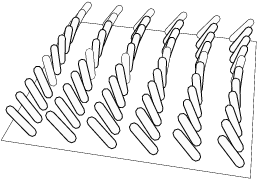
\includegraphics[width=65mm]{twistflat.1}
    \end{center}
    \caption{Figure that uses \myem{director\_invisible}
      and \myem{generatedirline}.}
  \end{figure}
}

\subsubsection{Surface Plots}

\FP\ surface plots are geared towards unusual features like
equilateral triangular grid, hexagonal domain and merging
together functional and parametric surface descriptions.
\begin{itemize}
\item draw {\bfseries hexagonaltrimesh()} Plots a
functional surface on a triangular or hexagonal
domain. Uses the \myem{LightSource}.
\begin{enumerate}
\item \myem{boolean} Select the kind of
domain. \myem{true} for hexagonal and
\myem{false} for triangular. The domain is
centered on the origin (\myem{black}). When the
domain is hexagonal two of its corners are on the
\myem{-YY} axis. When the
domain is triangular one of its corners is on the
\myem{X} axis. 
\item \myem{numeric} Number of small triangles on
each side of the triangular domain or three times
the number of small triangles on
each side of the hexagonal domain.
\item \myem{numeric} Length of the triangular
domain side or three times the hexagonal domain
side.
\item \myem{text} Name of the function that
returns the \myem{Z} coordinate of a surface
point of coordinates \myem{X} and \myem{Y}.
\end{enumerate}
\frame{
  \begin{figure}[bpt]
    \begin{center}
      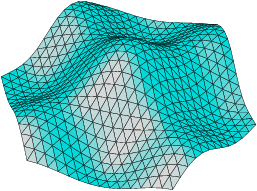
\includegraphics[width=65mm]{hexagonaltrimesh.1}
    \end{center}
    \caption{Figure that uses \myem{hexagonaltrimesh}.}
  \end{figure}
}
\item global {\bfseries partrimesh()} Defines a parametric
surface that can be drawn with
\myem{draw\_invisible}. In the following descriptions
\myem{S} and \myem{T} are the parameters. Remember
to initialize \myem{NF}. The surface is defined so
that quadrangles are used whenever possible. If
impossible, two triangles are used but their
orientation is selected to maximize the surface
smoothness. Also note that, unlike
\myem{hexagonaltrimesh()}, the spatial range you
require to be visible is always first reshaped into a
cube and second compressed or extended vertically. How
much the cube is compressed or extended depends on the
last \myem{numeric} argument, the compression factor
for \myem{Z}, meaning that the final height of the
cube is 2/(compression factor). Thanks to Sebastian
Sturm for pointing the need to explain this.
\begin{enumerate}
\item \myem{numeric} Number of \myem{T} steps.
\item \myem{numeric} Number of \myem{S} steps.
\item \myem{numeric} Minimal \myem{T} value.
\item \myem{numeric} Maximal \myem{T} value.
\item \myem{numeric} Minimal \myem{S} value.
\item \myem{numeric} Maximal \myem{S} value.
\item \myem{numeric} Minimal \myem{X} value.
\item \myem{numeric} Maximal \myem{X} value.
\item \myem{numeric} Minimal \myem{Y} value.
\item \myem{numeric} Maximal \myem{Y} value.
\item \myem{numeric} Minimal \myem{Z} value.
\item \myem{numeric} Maximal \myem{Z} value.
\item \myem{numeric} Compression factor for \myem{Z}
values.
\item \myem{text} Name of the function that
returns a surface point (of \myem{color} type)
for each pair (\myem{S},\myem{T}).
\end{enumerate}
\end{itemize}


\subsubsection{Strictly 2D}
\begin{itemize}
\item path {\bfseries springpath()}
  \begin{enumerate}
  \item \myem{pair} Start point.
  \item \myem{pair} Finish point.
  \item \myem{numeric} Number of swings.
  \item \myem{numeric} Half-width of the swings.
  \item \myem{numeric} Fraction of the length that is occcupied with swings.
  \end{enumerate}
\item path+draw {\bfseries zigzagfrontier()}
  \begin{enumerate}
  \item \myem{pair} Start point.
  \item \myem{pair} Finish point.
  \item \myem{numeric} Number of swings.
  \item \myem{numeric} Standart deviation of the swings' amplitude.
  \item \myem{numeric} Average swings' amplitude.
  \item \myem{numeric} Outside thickness.
  \item \myem{numeric} Inside thickness.
  \item \myem{colour} Outside color.
  \item \myem{colour} Inside color.
  \end{enumerate}
\item path {\bfseries randomcirc()}
  \begin{enumerate}
  \item \myem{numeric} Average radius. 
  \item \myem{numeric} Standart deviation.
  \item \myem{numeric} Number of points.
  \end{enumerate}
\item pair {\bfseries radialcross()} Calculates one of both
  intersections between to circles.
  \begin{enumerate}
  \item \myem{pair} Center of the first circle. 
  \item \myem{numeric} Radius of the first circle.
  \item \myem{pair} Center of the second circle.
  \item \myem{numeric} Radius of the second circle.
  \item \myem{boolean} Choice between the upside (\myem{true}) or
    downside (\myem{false}) intersection (relative to the segment
    connecting both centers). 
  \end{enumerate}
\item draw {\bfseries ropepattern()} Draws a (climbing) rope over a
  path (see figure \ref{ropes}).
  \begin{enumerate}
  \item \myem{path} The path.
  \item \myem{numeric} Width or thickness of the rope.
  \item \myem{numeric} Number of windings of each thread.
  \end{enumerate}
  
\frame{
  \begin{figure}[bpt]
    \begin{center}
      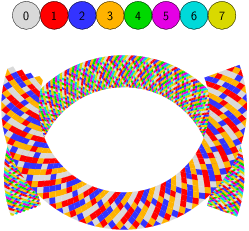
\includegraphics[width=65mm]{ropepatterns.1}
    \end{center}
    \caption{Figure that uses \myem{ropepattern}.}
    \label{ropes}
  \end{figure}
}
\item pair {\bfseries firsttangencypoint()} Returns the first point on
  a path for which the segment connecting that point and another given
  reference point is tangent to the path.
  \begin{enumerate}
  \item \myem{path} The path.
  \item \myem{pair} The reference point
  \item \myem{numeric} Reciprocal of the sampling step along the path
    in default units.
  \end{enumerate}
\item path {\bfseries lasermachine()} Shrink or swell a cyclic path
  without cusp points and without 
  coinciding pre and post control points. 
  \begin{enumerate}
  \item \myem{path} The original path.
  \item \myem{numeric} Directed distance between the original path and the
    returned path (positive values are to the right and negative
    values are to the left of the original path).
  \item \myem{numeric} Maximum cossine of corner angle above which it
    remains a sharp corner (only for negative values of directed distance).
  \end{enumerate}
\item path {\bfseries crossingline()} Produces a single path out of
  two intersecting and cyclic paths. The paths must be adapted with
  \myem{startahead} and/or \myem{reverse} so that they both rotate in the same
  direction and they start on consecutive "lobes".
  Now pay attention: given the direction of rotation (clockwise or
  counter-clockwise) the SecondPath must start BEFORE the FirstPath.
  And another problem: there must be at least four intersection points.
  \begin{enumerate}
  \item \myem{path} FirstPath.
  \item \myem{path} SecondPath.
  \item \myem{numeric} Time resolution.
  \end{enumerate}
\end{itemize}

\section{Missing documentation}
\begin{alltt}
minimizestep( expr Abcisscolor )( text PlainFunc )

improvertex( expr VerA, DisA, VerB, DisB, VerC, DisC, IniV )

ultraimprovertex( expr PlanPoi, PlanDir, BaseCenter, Radius, LenVec,
        CentrPoi, NorthPoleVec, Ray, IniV )

necplusimprovertex( expr PlanPoi, PlanDir,
	CentrPoiA, NorthPoleVecA, RayA,
        CentrPoiB, NorthPoleVecB, RayB, IniV )

intersectprolatespheroid( expr CentrPoi, NorthPoleVec, Ray,
        LinePoi, LineDir, IniV )

intersectorus( expr Tcenter, Tmoment, Bray, Sray, LinePoi, LineDir )

ellipsoid( expr Centr, AxOne, AxTwo, AxThr )

revolparab( expr BaseCenter, ParabTip, BaseRay )

pointinsidetorus( expr Point, Tcenter, Tmoment, Bray, Sray )
\end{alltt}



\mode<article>{\newpage}

\section{Reference-at-a-glance}

\subsection{Sphere}

\frame{
  \frametitle{\myem{tropicalglobe}( $N$, $\vec{c}$, $R$, $\vec{A}$ )}
  \begin{center}
    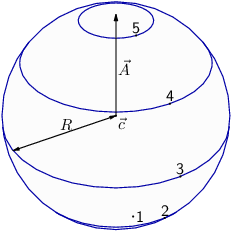
\includegraphics[width=65mm]{revolvers.1} \\
    
    \myem{tropicalglobe( 5, black, 1, blue );}
  \end{center}
}

\subsection{Disc}

\frame{
  \frametitle{\myem{rigorousdisc}( $R_i$, 
    \myem{bool}, $\vec{c}$, $R_o$, $\vec{A}$ )}
  \begin{center}
    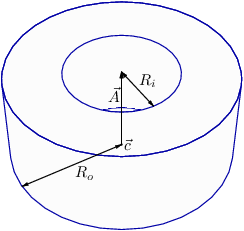
\includegraphics[width=65mm]{revolvers.2} \\

    \myem{rigorousdisc( 0.5, true, black, 1, 0.85blue );}
  \end{center}
}

\subsection{Torus}

\frame{
  \frametitle{\myem{smoothtorus}( $\vec{c}$, $\vec{A}$, $R_b$, $R_s$ )}
  \begin{center}
    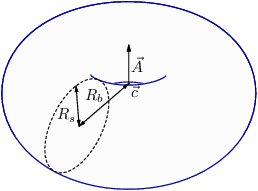
\includegraphics[width=65mm]{revolvers.3} \\

    \myem{smoothtorus( black, blue, 0.7, 0.4 );}
  \end{center}
}

\subsection{Bowl}

\frame{
  \frametitle{\myem{spatialhalfsfear}( $\vec{c}$, $\vec{A}$, $R$ )}
  \begin{center}
    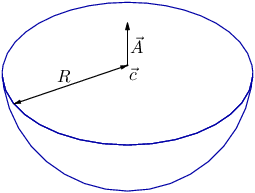
\includegraphics[width=65mm]{revolvers.4} \\

    \myem{spatialhalfsfear( black, blue, 1 );}
  \end{center}
}

\subsection{Cuboid}

\frame{
  \frametitle{\myem{kindofcube}(\myem{bool,bool},$\vec{o},\alpha_1,\alpha_2,\alpha_3,l_1,l_2,l_3$)}
  \begin{center}
    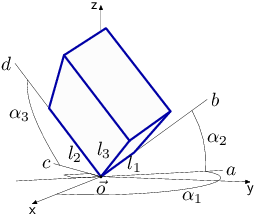
\includegraphics[width=65mm]{kindofcuber.1} \\

    \myem{kindofcube( false, true, black, 130, 32, 67, 0.3, 0.6, 0.9 );}
  \end{center}
}

\subsection{Simple car}

\frame{
  \frametitle{\myem{simplecar}( $\vec{o}$,($\alpha_1,\alpha_2,\alpha_3$),
    ($l_1,l_2,l_3$), (Xf,Yf,Zf), (Xr,Yr,Zr) )}
  \begin{center}
    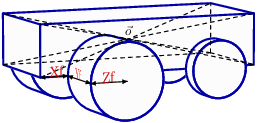
\includegraphics[width=65mm]{simplecarparam.1} \\

\myem{simplecar( black, black, (0.8,0.35,0.18), (0.1,0.2,0.132),
  (0.06,0.06,0.1) );}
  \end{center}
}

\subsection{Cone}

\frame{
  \frametitle{\myem{verygoodcone}( \myem{bool}, $\vec{c}$,
    $\vec{A}$, $R$, $\vec{v}$ )}
  \begin{center}
    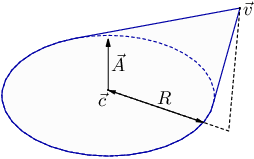
\includegraphics[width=65mm]{cone.1} \\

    \myem{verygoodcone( true, black, blue, 0.8, blue+green );}
  \end{center}
}

\subsection{Elliptic prism}

\frame{
  \frametitle{\myem{whatisthis}( $\vec{c}$, $\vec{S}_1$,
    $\vec{B}_1$, $D$, $||\vec{S}_2||/||\vec{S}_1||$ )}
  \begin{center}
    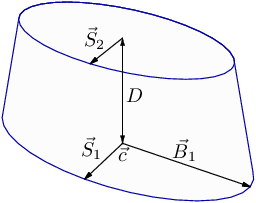
\includegraphics[width=65mm]{ellipticprism.1} \\
    
    \myem{whatisthis( black, 0.5red, green, 0.85, 0.8 );}
  \end{center}
}

\subsection{Spheroid}

\frame{
  \frametitle{\myem{spheroid}( $\vec{c}$, $\vec{S}$, $R$ )}
  \begin{center}
    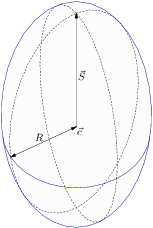
\includegraphics[width=40mm]{revolvers.5} \\

    \myem{spheroid( black, 2*blue, 1 );}
  \end{center}
}

\subsection{Cylindrical strip}

\frame{
  \frametitle{\myem{banana}( $\vec{c}$, $R$,
    $(\alpha_M,\beta_M,\gamma_M)$, $L$, $\theta$ )}
  \begin{center}
    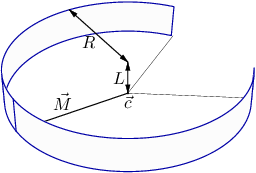
\includegraphics[width=70mm]{revolvers.6} \\

    \myem{banana( black, 1, black, 0.3, 145 );}
  \end{center}
}

\subsection{Torus' slice}

\frame{
  \frametitle{\myem{quartertorus}( $\vec{c}$, $\vec{A}$, $\vec{B}$, $R$ )}
  \begin{center}
    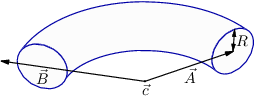
\includegraphics[width=70mm]{revolvers.7} \\

    \myem{quartertorus( black, -red, red-green, 0.25 );}
  \end{center}
}

\section{References}

\begin{description}
\item[1.] ``The \MF book'' by Don Knuth
\item[2.] ``\MP, a user’s manual'' by John Hobby and the
  MetaPost development team
\item[3.] ``The NURBSbook'' by Les Piegl and Wayne Tiller
\end{description}

\section{Acknowledgements}

\frame{
  \changeableframetitle{Acknowledgements}
  Many people have contributed to make \FP\ what it is today.
  Perhaps it would have never come into being without the early
  intervention of Jorge B\'arrios, providing access to his father's
  computer in 1986. Another important moment happened when Jos\'e Esteves 
  first spoke about \MP\ sometime in the late nineties.

  Also, the very accurate criticism of Cristian Barbarosie has
  significantly contributed to fundamental improvements. Jens
  Schwai\-ger contributed new macros. Pedro Sebas\-ti\~ao, Jo\~ao Dinis and
  Gon\-\c{c}alo Mo\-rais proposed challenging new features. 
}
\end{document}

